\documentclass[../main/Notes.tex]{subfiles}
\begin{document}

\section[Choice Models I]{Choice Models I \iftoggle{showdates}{\small{\textit{2014-07-04}}}{}}\index{Choice model}

\subsection*{Utility}\index{Utility}
\begin{wrapfigure}{r}{.3\textwidth}
   \centering
  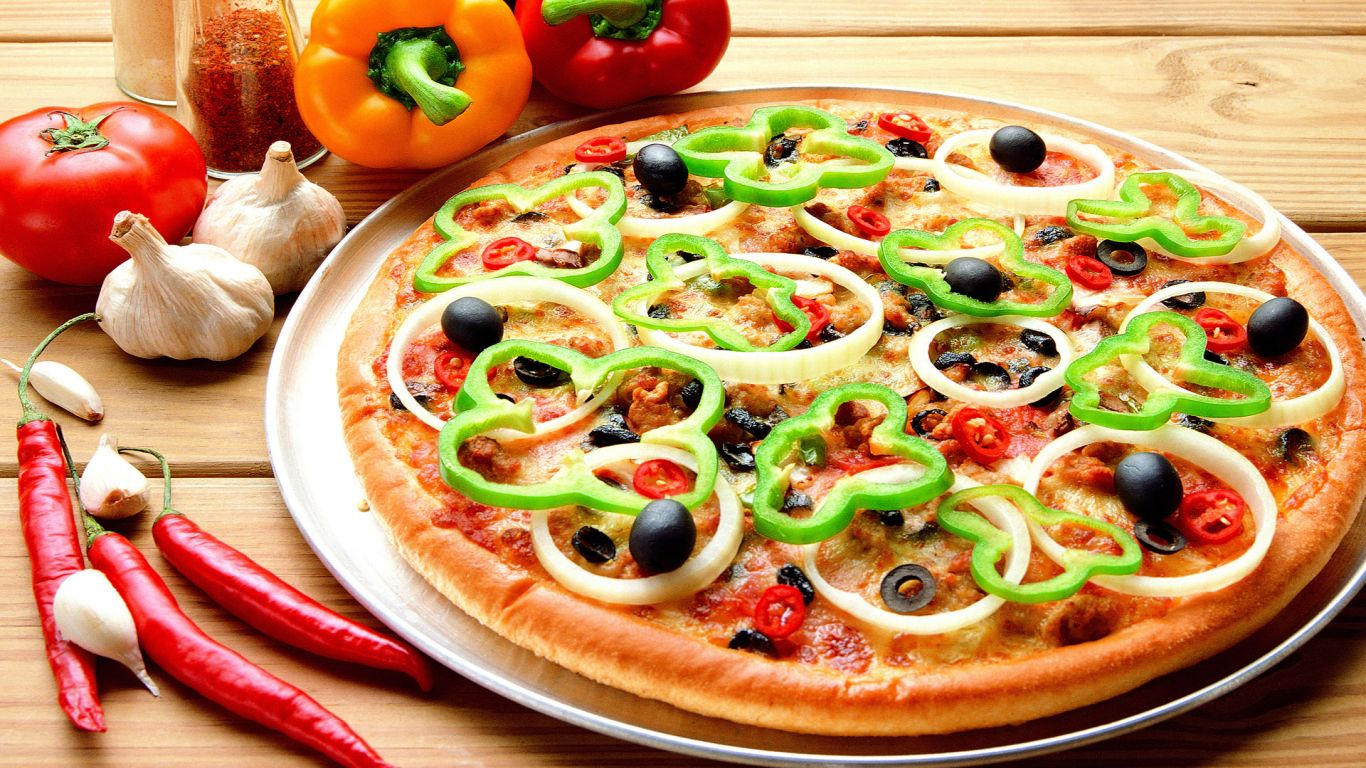
\includegraphics[width=.3\textwidth]{../images/pizza-free-wallpaper_1366x768_82178.jpg}
  \caption{Pizzaaaa!}
  \label{fig:2014-07-04-pizza}
\end{wrapfigure}
The \emph{utility} is the variability in choices. It can either refer to the variability in choices of several subjects (``How many subjects prefer pizza tonno over pizza salami?'') or the variability in choices of a single subject over time (``On how many days prefers the subject pizza tonno over pizza salami?''). A utility of e.g. 70\% means that a subject chooses pizza tonno over pizza salami in 70 out of 100 times it's asked.

With choice models we try to find the utility of possible choices in order to make accurate predictions.

Note that there might be \emph{polarizing} options, this means the variance changes. For example pizza margarita might be very popular, so many people like it thus the variance for a choice of pizza margarita gets smaller. However, pizza salami might be less popular and therefor its utility's variance is wider (see figure \ref{fig:2014-07-04-polarizing}.

Since the utility is dependent on the choice to made, there can only be \emph{relative} utilities.
\begin{figure}
\centering
\begin{tikzpicture}
  \begin{axis}[every axis plot post/.append style={mark=none, domain=-2:8, samples=50, smooth}, 
    axis x line*=bottom, axis y line*=left, enlargelimits=upper,yticklabels={},xticklabels={}]
    \addplot [red]    {gauss(0,0.5)};
      \addlegendentry{Pizza Margarita}
    \addplot [green]  {gauss(4,2)};
      \addlegendentry{Pizza Salami}
  \end{axis}
\end{tikzpicture}
\caption{Red: Pizza margarita is quite popular among all subjects. Green: Pizza salami is not that popular among subjects, it has a higher variance.}
\label{fig:2014-07-04-polarizing}
\end{figure}

\subsection{Paired Comparison Experiment}\index{Paired Comparison Experiment}
A very common technique to check whether subjects prefer an option over another is a paired comparison experiment. Subjects are shown \emph{all possible pairs} and say for each pair which option they prefer. This results in a matrix where we can find out which options are more popular than others. See table \ref{tab:2014-07-04-example_paired_comp_exp} for an example.

% todo: make this table more beautiful
\begin{table}
\centering
\begin{tabular}{l|c|c|c|}
\multicolumn{1}{l}{\rotatebox{45}{are chosen}} & \multicolumn{3}{c}{over these options} \\ \cline{2-4}\rule[-2.5ex]{0pt}{7ex}
\multirow{3}{1em}{\rotatebox{90}{these options}} & --- & $\frac{15}{60}$ & $\frac{40}{60}$ \\ \cline{2-4}\rule[-2.5ex]{0pt}{7ex}
& $\frac{45}{60}$ & --- & $\frac{30}{60}$ \\  \cline{2-4}\rule[-2.5ex]{0pt}{7ex}
& $\frac{20}{60}$ & $\frac{30}{60}$ & --- \\ \cline{2-4}
\end{tabular}
\caption{Example paired comparison outcome. In this example we assume we asked 60 subjects, hence the denominator.\\For computations we often set the diagonal (compare each option with itself) to $\frac{1}{2}$, which means there is no preference -- this already makes sense intuitively.}
\label{tab:2014-07-04-example_paired_comp_exp}
\end{table}

\subsubsection*{Two options}
\sidenote{To make it easier to understand the math we will assume equal variance for given options unless noted otherwise.}
Assume we ask a subject to make a choice between two options. We consider two options $i$ and $j$ with the random variables $x_i$ and $x_j$ as their utilities (the subject's utilities for each option respectively) with $x_i \sim \mathcal{N}\left(\mu_i,1\right)$ and $x_j \sim \mathcal{N}\left(\mu_j,1\right)$. The subject ``computes'' $\Delta x_{ij} = x_i - x_j$ if $\Delta x_{ij} > 0$ (otherwise we would need $\Delta x_{ji}$). $\Delta x_{ij}$ is also normal distributed, i.e. $\Delta_x{ij} \sim \mathcal{N}\left(\mu_i-\mu_j,2\right)$. $\Delta x_{ij}$ is the distribution of how likely it is, that the subject chooses $i$ over $j$. A visualization of this can be found in figure \ref{fig:2014-07-04-compute_delta_xij}.

\begin{figure}
\centering
\begin{tikzpicture}
	\begin{axis}[domain=-2:6, enlargelimits=upper, axis x line*=bottom, axis y line*=left]
    \addplot [red,samples=50]   {gauss(1,1)};
      \addlegendentry{$x_j$};
    \addplot [green,samples=50] {gauss(3,1)};
      \addlegendentry{$x_i$};
    \addplot [blue,samples=50]  {gauss(2,2)};
      \addlegendentry{$\Delta x_{ij}$};
  \end{axis}
\end{tikzpicture}
\begin{tikzpicture}
  \begin{axis}[domain=-2:8, enlargelimits=upper, axis x line*=bottom, axis y line*=left]
    \addplot [red,samples=50]   {gauss(1,0.75)};
      \addlegendentry{$x_j$};
    \addplot [green,samples=50] {gauss(4,1.5)};
      \addlegendentry{$x_i$};
    \addplot [blue,samples=50]  {gauss(3,2.25)};
      \addlegendentry{$\Delta x_{ij}$};
  \end{axis}
\end{tikzpicture}
\caption{Relation of $x_i, x_j$ and $\Delta x_{ij}$. Left: two options with equal variance. Right: two options with different variances. Note that the variances add up, hence $\Delta x_{ij}$ gets flat and wide.}
\label{fig:2014-07-04-compute_delta_xij}
\end{figure}

\begin{figure}
  \centering
  \begin{tikzpicture}
    \begin{axis}[domain=-5:2, enlargelimits=upper, axis x line*=bottom, axis y line*=left]
      \addplot+[domain=0:2, samples=100, pattern=flexible hatch, mark=none
                hatch distance=5pt, hatch thickness=0.5pt,
                draw=green, pattern color=green!40, area legend]
                {gauss(-3,2)} \closedcycle;
        \addlegendentry{$\int\limits_0^\infty\Delta x_{ij}$}
      \addplot[domain=-5:2, samples=50, red] {gauss(-3,2)};
        \addlegendentry{$\Delta x_{ij}$}
      \draw[-,below] (axis cs:0,0)--(axis cs:0,1) node{0};
      \draw[-,dashed,above] (axis cs:0.5,0.025)--(axis cs:1,0.1) node{$\mathcal{A}$};
      \draw[-,dotted,above] (axis cs:-3,-0.01)--(axis cs:-3,0.2) node{$\mu_i-\mu_j$};
    \end{axis}
  \end{tikzpicture}
  \caption{$\Delta x_{ij}$: If we know this area $\mathcal{A}$, we can guess $\Delta \mu_{ij}$.}
  \label{fig:2014-07-04-guessing_delta_mu}
\end{figure}

\subsubsection*{Definitions}
We define:
\begin{itemize}
	\item $d_{ij} = \mu_i-\mu_j$
  \item $p_{ij}$ is the probability that the subject chooses $i$ over $j$.
  \item $P_{ij} = 1-P_{ji} = 1-\Phi(d_{ij};0,\sqrt{2}) = 1-\Phi(-d_{ij};0,\sqrt{2}) \stackrel{\text{\footnotesize z-tf.}}{=} 1-\Phi\left(-\frac{d_{ij}}{\sqrt{2}};0,1\right)$
     \\ Figure \ref{fig:2014-07-04-Phi0} shows visually that $\Phi(x)=1-\Phi(-x)$, so we can write $1-\Phi\left(-\frac{d_{ij}}{\sqrt{2}};0,1\right) = \Phi\left(\frac{d_{ij}}{\sqrt{2}};0,1\right)$.
     \\ To further simplify the notation we just write $\Phi\left(\frac{d_{ij}}{\sqrt{2}}\right)$.
  \item $q_{ij}$
\end{itemize}

\begin{figure}
  \centering
  \begin{tikzpicture}
    \begin{axis}[restrict x to domain=-2:2, restrict y to domain=0:1.1, enlargelimits=false, axis x line*=bottom, axis y line*=left, legend style={at={(1,0.5)},anchor=east}]
      \addplot[mark=none,red,samples=50,domain=-2:2]{Gauss(0,1)};
        \addlegendentry{$\Phi(x)$}
      \addplot[mark=none,blue,samples=50,domain=-2:2]{(1/(1+exp(-0.07056*(-x)^3-1.5976*(-x)))};
        \addlegendentry{$\Phi(-x)$}
    \end{axis}
  \end{tikzpicture}
  \caption{$\Phi(x)=1-\Phi(-x)$}
  \label{fig:2014-07-04-Phi0}
\end{figure}

\subsection*{Optimizing Paired Comparison Experiment}
We search for an estimate of $d_{ij}$. We can use $q_{ij} = \Phi\left(\frac{\est{d_{ij}}}{\sqrt{2}}\right)$ and derive $\Phi^-1\left(q_{ij}\right) = \frac{\est{d_{ij}}}{\sqrt{2}} \Leftrightarrow \sqrt{2}\Phi^{-1}\left(q_{ij}\right) = \est{d_{ij}}$.

\sidenote{$\forall i\!: \est{d_{ii}}=0$}
$\est{d}$ is a matrix (figure \ref{fig:2014-07-04-est_d_exp}) with the estimated distances for $\est{d_{ij}} = \est{\mu_i}-\est{\mu_j}$. Hence $\est{d_{ij}}=-\est{d_{ji}}$. But what are good estimates for $\est{\mu_i}$ and $\est{\mu_j$}?

\begin{figure}[hb]
  \centering
  \begin{align*}
    \est{d}=\left( \begin{array}{ccccc}
      0            &   & \cdots & \est{d_{ij}} &  \\
                   & 0 &        &              &  \\
      \vdots       &   & 0      &              & \vdots \\
      \est{d_{ji}} &   &        & 0            &  \\
                   &   & \cdots &              & 0 
    \end{array} \right)
  \end{align*}
  \caption{$\est{d}$, note that $d_{ji} = -d_{ij}$ and the diagonal is 0.}
  \label{fig:2014-07-04-est_d_exp}
\end{figure}

We have $\frac{n(n-1)}{2}$ pairs, that means we have $(n-1)$ free parameters. This means we will not be able to determine the x-shift. This shouldn't bother us too much, since we are only interested in the difference between $\mu_i$ and $\mu_j$ anyway.

A method for minimizing (thus optimizing) the error in our estimates we can use the least squares estimate (LSE)\index{Least Squares Estimate}.

\subsection{Least Squares Estimate}\index{Least Squares Estimate}
The idea of the least squares estimate is to \emph{minimize the sum of all squared differences}.
\begin{align*}
Q = \frac{1}{2}\left( \sum\limits_j \sum\limits_i \left( \est{\mu_i}-\est{\mu_j} - \est{d_{ij}} \right) \right)
\end{align*}
So we want to minimize $Q$ with respect to $\est{\mu_i}$ and $\est{\mu_j}$. 

This can be done easily by taking the first derivative and setting it to 0.
\begin{align*}
\frac{\partial Q}{\partial \est{\mu_k}} &=             \left( \sum\limits_j \est{\mu_k} - \est{\mu_j} - \est{d_{kj}} \right) - \left( \sum\limits_i \est{\mu_i} - \est{\mu_k}              - \est{d_{ik}} \right) = 0\\
                          &\Leftrightarrow             \left( \sum\limits_j \est{\mu_k} - \est{\mu_j} - \est{d_{kj}} \right) + \left( \sum\limits_i \est{\mu_k} - \est{\mu_i} \underbrace{ + \est{d_{ik}} }_{\text{Remember: }d_{ij}=-d{ji}} \right) = 0\\
                          &\Leftrightarrow \underbrace{\left( \sum\limits_j \est{\mu_k} - \est{\mu_j} - \est{d_{kj}} \right) + \left( \sum\limits_i \est{\mu_k} - \est{\mu_i}              - \est{d_{ki}} \right)}_{\text{twice the same}} = 0\\
                          &\Leftrightarrow           2 \left( \sum\limits_i \est{\mu_k} - \est{\mu_i} - \est{d_{ki}} \right) = 0\\
                          &\Leftrightarrow                    \sum\limits_i \est{\mu_k} - \est{\mu_i} - \est{d_{ki}}         = 0\\
                          &\Leftrightarrow    n \est{\mu_k} -            \sum\limits_i \est{\mu_i} -            \sum\limits_i \est{d_{ki}} = 0 \\
                          &\Leftrightarrow      \est{\mu_k} - \frac{1}{n}\sum\limits_i \est{\mu_i} = \frac{1}{n}\sum\limits_i \est{d_{ki}}
\end{align*}
We end up with $n$ equations (one for each $k$) in $n$ unknowns. However the system's rank is $n-1$, so the system of equations is underdetermined. This means that to solve it we are free to choose something as we want, and obviously we set the average of the $\mu_i$s to 0 and get a nice formula to calculate the average over all distances, $\est{\mu_k}$.
\begin{align*}
\frac{1}{n} \sum\limits_i \est{d_{ki}} \stackrel{!}{=} 0 \Rightarrow \est{\mu_k} = \frac{1}{n} \sum\limits_i \est{d_{ki}}
\end{align*}

\subsubsection*{Simple example}
We have three normal distributions $i, j,$ and $k$ with the means $\mu_i = 1, \mu_j = 0,$ and $\mu_k = -1$ (figure \ref{fig:2014-07-04-normaldists}).
\begin{figure}[htb]
  \centering
  \begin{tikzpicture}
    \begin{axis}[enlargelimits=false, restrict x to domain=-2:2, mark=none, axis x line*=bottom, axis y line*=left]
      \addplot[red, samples=100]   {gauss(1,1)};
        \addlegendentry{$i$}
      \addplot[green, samples=100] {gauss(0,1)};
        \addlegendentry{$j$}
      \addplot[blue, samples=100]  {gauss(-1,1)};
        \addlegendentry{$k$}
    \end{axis}
  \end{tikzpicture}
  \caption{Three normal distributions $i, j,$ and $k$.}
  \label{fig:2014-07-04-normaldists}
\end{figure}

For these distributions we can simply derive the matrix $d$ and calculate the average distance between two plots.

\begin{align*}
d = \left( \begin{array}{ccc}
 0 &  1 & 2 \\
-1 &  0 & 1 \\
-2 & -1 & 0
\end{array} \right)
\end{align*}

\begin{align*}
\mu_i = \frac{1}{n} \sum\limits_l d_{il} = \frac{1}{3} \left( d_{i1} + d_{i2} + d_{i3} \right) = \frac{1}{3} \left( 0 + 1 + 2 \right) = 1
\end{align*}



\subsection{Thurstone Scaling}

\subsection{Weak Stochastic Transitivity}

\subsection{Strong Stochastic Transitivity}

\subsection{Restle's Choice Model}





\end{document}